\chapter{Stationary black holes}
\label{s:sta}

\minitoc

\section{Introduction}

\section{Definition and first properties} \label{s:sta:def_station}

Let us consider a spacetime $(\M,\w{g})$ that contains a black hole, as defined in
Sec.~\ref{s:glo:def_BH}. In particular, $(\M,\w{g})$ admits a future null
infinity $\scri^+$ and a past null infinity $\scri^-$. One says that
$(\M,\w{g})$ is a \defin{stationary spacetime}\index{stationary!spacetime}
if (i) it is invariant under
the action of the translation group $(\mathbb{R},+)$ and (ii) the orbits of
the group action are timelike curves in the vicinity of $\scri^+$ and
$\scri^-$. It is equivalent to say that there exists a Killing vector field
$\w{\xi}$ (the generator of the translation group, cf. Sec.~\ref{s:neh:symmetries}) that is timelike in the vicinity of $\scri^+$ and $\scri^-$.

\begin{remark}
Some authors (e.g. Carter \cite{Carte73b}) call such spacetimes
\emph{pseudo-stationary}\index{pseudo-stationary}, keeping the qualifier
\emph{stationary} for the case where the Killing field $\w{\xi}$ is timelike
in all $\M$. As we going to see, when $\M$
contains a black hole, $\w{\xi}$ cannot be timelike everywhere,
so only \emph{pseudo-stationarity} in the above sense is relevant for them.
Our terminology follows that of Chru\'sciel, Lopes Costa \& Heusler \cite{ChrusLH12}
and Choquet-Bruhat \cite{Choqu09}.
\end{remark}

If $(\M,\w{g})$ is invariant under the action of the isometry group $(\mathbb{R},+)$,
so is $\scri^+$ (under some proper extension of $\w{\xi}$ to the conformal
completion $\tilde{\M}$)
and therefore its causal past $J^-(\scri^+)$. As the boundary of $J^-(\scri^+)$
inside $\M$, the event horizon $\Hor$ must therefore be invariant under the
action of the isometry group.
Note that this means that $\Hor$ is invariant \emph{as a whole}, not that
each point of $\Hor$ is invariant under the group action.
Now, $\Hor$ is globally invariant if, and only if, the
generator $\w{\xi}$ of the isometry group is tangent to $\Hor$.
Let us assume that $\Hor$ is smooth (which sounds likely in a stationary context;
a rigorous proof can be found in \cite{ChrusDGH01}),
it is then a null hypersurface (Property~4 in Sec.~\ref{s:glo:properties_H}).
Since a timelike vector cannot be tangent to a null hypersurface (cf. the
lemma in Sec.~\ref{s:def:spacelike_sections}), we conclude that
\begin{greybox}
In a stationary spacetime containing a black hole,
the stationary Killing vector field  $\w{\xi}$ is tangent to the event horizon
$\Hor$, which implies that $\w{\xi}$ is either null or spacelike on $\Hor$.
\end{greybox}

\section{The event horizon as a Killing horizon}

Let us discuss successively the two allowed types for the stationary
Killing vector $\w{\xi}$ on $\Hor$: null and spacelike.

\subsection{Null stationary Killing field on $\Hor$: the staticity theorem}

By the lemma of Sec.~\ref{s:def:spacelike_sections}, if the Killing vector
field $\w{\xi}$ is null on $\Hor$, it is necessarily tangent to the null geodesic generators
of $\Hor$ and therefore collinear to the null normals $\wl$ of $\Hor$. From the definition
given in Sec.~\ref{s:neh:def_Killing_hor}, it follows immediately that
$\Hor$ is a Killing horizon (with respect to the Killing field $\w{\xi}$).
In dimension $n=4$ and using the Einstein equation,
D.~Sudarski and R.M.~Wald (1992) \cite{SudarW92} have then proven that $\w{\xi}$ must be
hypersurface-orthogonal everywhere, i.e. that the spacetime $(\M,\w{g})$ is \defin{static}\index{static spacetime}. For this reason, Sudarski \& Wald's result is often
called the \defin{staticity theorem}\index{staticity theorem}.

Having that $(\M,\w{g})$ is static, we can go further and
apply the
\begin{greybox}[frametitle={Israel uniqueness theorem:}]
\index{Israel uniqueness theorem}
If $(\M,\w{g})$ is a $n$-dimensional static spacetime
containing a black hole, with $\w{g}$ solution of the vacuum Einstein
equation, then the domain of outer communications of $\M$ is isomorphic
to the domain of outer communications of a $n$-dimensional Schwarzschild spacetime\index{Schwarzschild!spacetime}.
\end{greybox}
This theorem has been proved in 1967 by W.~Israel \cite{Israe67},
and improved latter by many authors (in particular by
P. Chru\'sciel \& G. Galloway (2010) \cite{ChrusG10}, who removed
the hypothesis of analyticity).
A demonstration of Israel's theorem can be found in Straumann's textbook \cite{Strau04}.

So basically, in dimension $n=4$ (i.e. when the staticity theorem applies), all stationary vacuum black holes with the stationary Killing field $\w{\xi}$ null
on $\Hor$ are nothing but Schwarzschild black holes, which we will study in detail in Chap.~\ref{s:sch}.


\subsection{Spacelike stationary Killing field on $\Hor$: the strong rigidity theorem}
\label{s:sta:strong_rigidity}

When $\w{\xi}$ is spacelike on $\Hor$, it obviously cannot be collinear to
any null normal $\wl$ of $\Hor$.
Assuming that $\Hor$ has cross-sections of spherical topology, we observe
that, with respect to the null geodesic generators of $\Hor$, the field lines of $\w{\xi}$
form some helices (cf. Fig.~??). By reciprocity, with respect to the field lines of $\w{\xi}$,
the null geodesic generators form some helices as well (cf. Fig.~??).
Since asymptotically the field lines of $\w{\xi}$ are worldlines of inertial observers,
we may say (in loose terms at this stage) that the event horizon $\Hor$
``is rotating'', all the more that we have seen above that when the null
generators coincide with the field lines of $\w{\xi}$, the black hole is static, i.e. non-rotating.

Since the Killing field $\w{\xi}$ is not null on $\Hor$, we cannot say a priori
that $\Hor$ is a Killing horizon. However, it turns out
that this is indeed the case, according to a famous result by S.W.~Hawking (1972)
\cite{Hawki72,HawkiE73}, known as the
\defin{strong rigidity theorem}\index{strong!rigidity theorem}\index{rigidity theorem!strong --}.
Assuming $n=4$ and the metric $\w{g}$ obeying the vacuum Einstein equation,
Hawking was able to show that there exists a second Killing vector field,
$\w{\chi}$ say, which is null on $\Hor$. Hence $\Hor$ is a Killing horizon
in this case as well, albeit not with respect to the
stationary Killing vector field $\w{\xi}$.

Hawking's result has been extended to dimensions $n\geq 4$ by V.~Moncrief
and J.~Isenberg (2008) \cite{MoncrI08}, under the hypotheses that $\Hor$
has cross-sections that are compact and transverse to $\w{\xi}$ (see also
Theorem~8.1 p.~470 of Choquet-Bruhat's textbook \cite{Choqu09}).
Both Hawking's result
and Moncrief \& Isenberg's one rely on the rather strong assumption that $\M$ and $\Hor$
are (real) \emph{analytic} manifolds, with $\w{g}$ being an analytic field. On physical grounds,
it would be desirable to assume only \emph{smooth} manifolds and fields.
Recently, S.~Alexakis, A.D.~Ionescu and S.~Klainerman \cite{AlexaIK14} (2014)
have succeeded in proving the strong rigidity theorem without the analyticity
assumption, but only for slowly rotating black holes.

Since we have two Killing vectors, $\w{\xi}$ and $\w{\chi}$, we may
form any linear combination of them with constant coefficients
and still get a Killing vector. For instance, if $\Omega_H$ is a non-zero constant,
the vector field $\w{\eta}$ defined by
\be
    \w{\eta} = \frac{1}{\Omega_H} \left( \w{\chi} - \w{\xi} \right)
    \quad\iff\quad
    \w{\chi} = \w{\xi} + \Omega_H \w{\eta} ,
\ee
is a Killing vector field on $\M$.
One can show (see e.g. \cite{Chrus97} for a rigorous proof) that $\Omega_H$
and some constant rescaling of $\w{\chi}$
can be chosen so that $\w{\eta}$ is a spacelike vector field whose
field lines are closed, with $2\pi$-periodicity in terms of the parameter $\ph$
associated to $\w{\eta}$ (i.e. $\w{\eta} = \D/\D\ph$ along the field lines),
and such that $\w{\eta}$ vanishes on a timelike 2-dimensional surface, called
the \defin{rotation axis}\index{rotation!axis}.
It follows that
the isometry group whose generator is $\w{\eta}$ is the rotation group
$\mathrm{SO}(2)$. In other words, the spacetime $(\M,\w{g})$ is
\defin{axisymmetric}\index{axisymmetric!spacetime} in addition to be stationary.
The constant $\Omega_H$ is then called the
\defin{black hole rotation velocity}\index{black hole!rotation velocity}\index{rotation!velocity}.

By the very definition of stationarity, the Killing vector field $\w{\xi}$ is
timelike in the vicinity of $\scri^+$ and $\scri^-$. If $\w{\xi}$ is spacelike
on $\Hor$, as assumed in this section, by continuity it must be spacelike
in some part of the domain of outer communications $\langle\langle \M\rangle\rangle$
near $\Hor$. The simplest configuration is then when
$\w{\xi}$ is spacelike in some connected region $\mathscr{G}\subset \langle\langle \M\rangle\rangle$
around $\Hor$, null at the boundary of $\mathscr{G}$ and timelike outside $\mathscr{G}$
up to $\scri^+$ and $\scri^-$ (cf. Fig.~??). The subset $\mathscr{G}$ is
called the \defin{ergoregion}\index{ergoregion} and its boundary $\E:=\partial\mathscr{G}$
the \defin{ergosphere}. We shall discuss it further in connection with
the Penrose process in Chap.~\ref{s:ker}.

%%%%%%%%%%%%%%%%%%%%%%%%%%%%%%%%%%%%%%%%%%%%%%%%%%%%%%%%%%%%%%%%%%%%%%%%%%%%%%%


\section{Bifurcate Killing horizons} \label{s:sta:bifur_Killing_hor}

\subsection{Definition and first properties}

Let $(\M,\w{g})$ be a $n$-dimensional spacetime endowed with a Killing vector
field $\w{\xi}$. A
\defin{bifurcate Killing horizon}\index{bifurcate!Killing horizon}\index{Killing!horizon!bifurcate --}\index{horizon!bifurcate Killing --} is the
union
\be
    \Hor = \Hor_1 \cup \Hor_2 ,
\ee
with the following properties:
\begin{itemize}
\item $\Hor_1$ and $\Hor_2$ are two null hypersurfaces;
\item $\Sp:=\Hor_1\cap\Hor_2$ is a spacelike $(n-2)$-surface;
\item each of the sets $\Hor_1\setminus\Sp$ and $\Hor_2\setminus\Sp$ has two connected components, which are
Killing horizons\footnote{Cf. Sec.~\ref{s:neh:def_Killing_hor} for the
definition of a Killing horizon.} with respect to $\w{\xi}$.
\end{itemize}
The $(n-2)$-dimensional submanifold $\Sp$ is called the
\defin{bifurcation surface}\index{bifurcation!surface} of $\Hor$.

\begin{figure}
\centerline{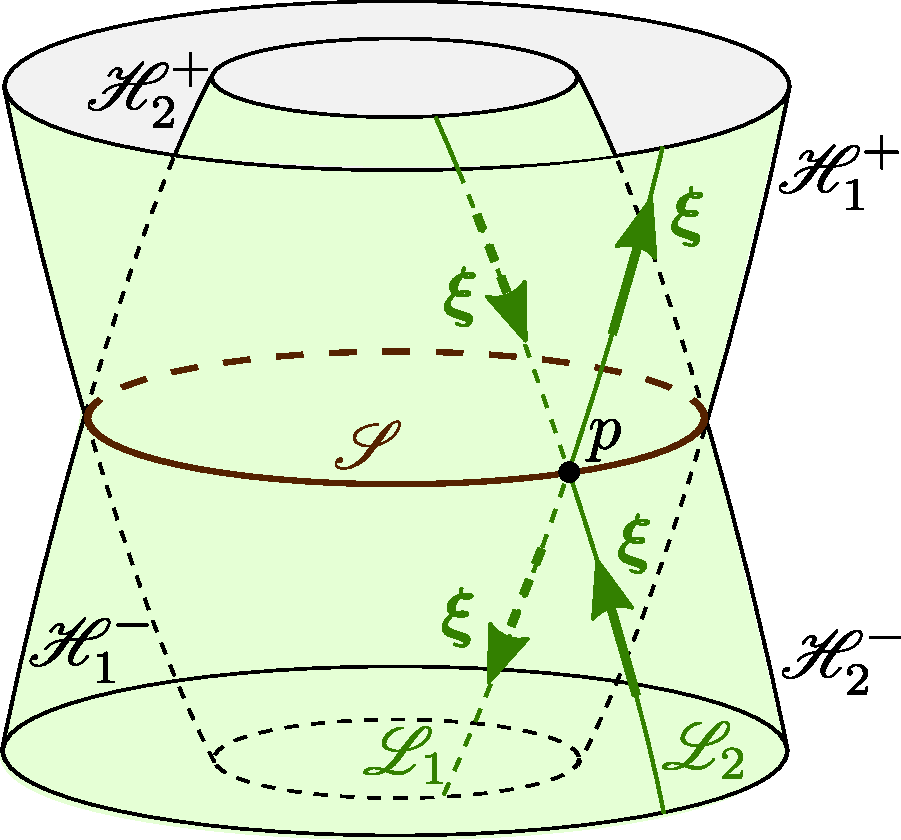
\includegraphics[width=0.5\textwidth]{sta_bifur_Kill_hor.pdf}}
\caption[]{\label{f:sta:bifur_Kill_hor} \footnotesize
Bifurcate Killing horizon $\Hor_1\cup\Hor_2$ with respect to the Killing vector
field $\w{\xi}$; $\Sp$ is the bifurcation surface. $\Li_1$ and $\Li_2$ are
null geodesic generators of respectively $\Hor_1$ and $\Hor_2$, which cross
each other at the point $p\in\Sp$.}
\end{figure}

Hence we may say that a bifurcate Killing horizon is formed by four Killing horizons,
$\Hor_1^+$, $\Hor_1^-$, $\Hor_2^+$ and $\Hor_2^-$ say,
which are merged together at the bifurcation surface $\Sp$ (cf. Fig.~\ref{f:sta:bifur_Kill_hor}), in such a way that
\[
    \Hor_1 = \Hor_1^- \cup \Sp \cup \Hor_1^+ \quad \mbox{and}\quad
    \Hor_2 = \Hor_2^- \cup \Sp \cup \Hor_2^+
\]
are null hypersurfaces.

A first property of bifurcate Killing horizons is
\begin{greybox}
The Killing vector field vanishes on the bifurcation surface:
\be
    \encadre{\left. \w{\xi} \right| _{\Sp} = 0 } .
\ee
\end{greybox}
\begin{proof}
Let $p\in \Sp$ and let us assume that $\left.\w{\xi}\right| _p\not=0$.
Let $\Li_1$ (resp. $\Li_2$) be the null geodesic generator of $\Hor_1$
(resp. $\Hor_2$) that intersects $\Sp$ at $p$ (cf. Fig.~\ref{f:sta:bifur_Kill_hor}).
Since $\Sp$ is spacelike,
$\Li_1$ and $\Li_2$ are unique. By definition of a Killing horizon,
$\w{\xi}$ is tangent to $\Li_1\cap\Hor_1^+$ and to $\Li_1\cap\Hor_1^-$,
i.e. to $\Li_1\setminus\{p\}$.
If $\left.\w{\xi}\right| _p \not=0$, then by continuity,
$\w{\xi}$ is a (non-vanishing) tangent vector field all along $\Li_1$.
Similarly, $\w{\xi}$ is tangent to all $\Li_2$.
At their intersection point $p$, $\Li_1$ and $\Li_2$ have then a common tangent
vector, namely $\left.\w{\xi}\right| _p$. Since $\Li_1$ and $\Li_2$ are
geodesics, this implies $\Li_1 = \Li_2$. Then
$\Li_1 \subset \Hor_1 \cap \Hor_2 = \Sp$. But since $\Sp$ is spacelike and
$\Li_1$ is null, we reach a contradiction. Hence we must have
$\left.\w{\xi}\right| _p = 0$.
\end{proof}

\begin{remark}
\label{r:sta:zero_Killing}
Having a Killing vector field that vanishes somewhere (here $\Sp$) is not the sign
of any pathology: it simply means that the points of $\Sp$ are invariant
by the isometries generated by $\w{\xi}$:
setting $\w{\xi}=0$ in Eq.~(\ref{e:neh:xi_dxdt}) leads to $\D\w{x}=0$, i.e.
to $\Phi_{\D t}(p) = p$.
\end{remark}

\begin{remark}
Contrary to what the name may suggest, a bifurcate Killing horizon is \emph{not}
a Killing horizon, for the latter, as defined in Sec.~\ref{s:neh:def_Killing_hor},
is a regular (i.e. embedded) hypersurface
of $\M$ (cf. Sec.~\ref{s:bas:embed} in Appendix~\ref{s:bas}), while
the union of two hypersurfaces is not in general a hypersurface. Moreover
on a Killing horizon, the Killing vector field is nowhere vanishing
[cf. Eq.~(\ref{s:neh:xi_on_KH})], while on
a bifurcate Killing horizon, it is vanishing at the bifurcation surface.
\end{remark}

\begin{figure}
\centerline{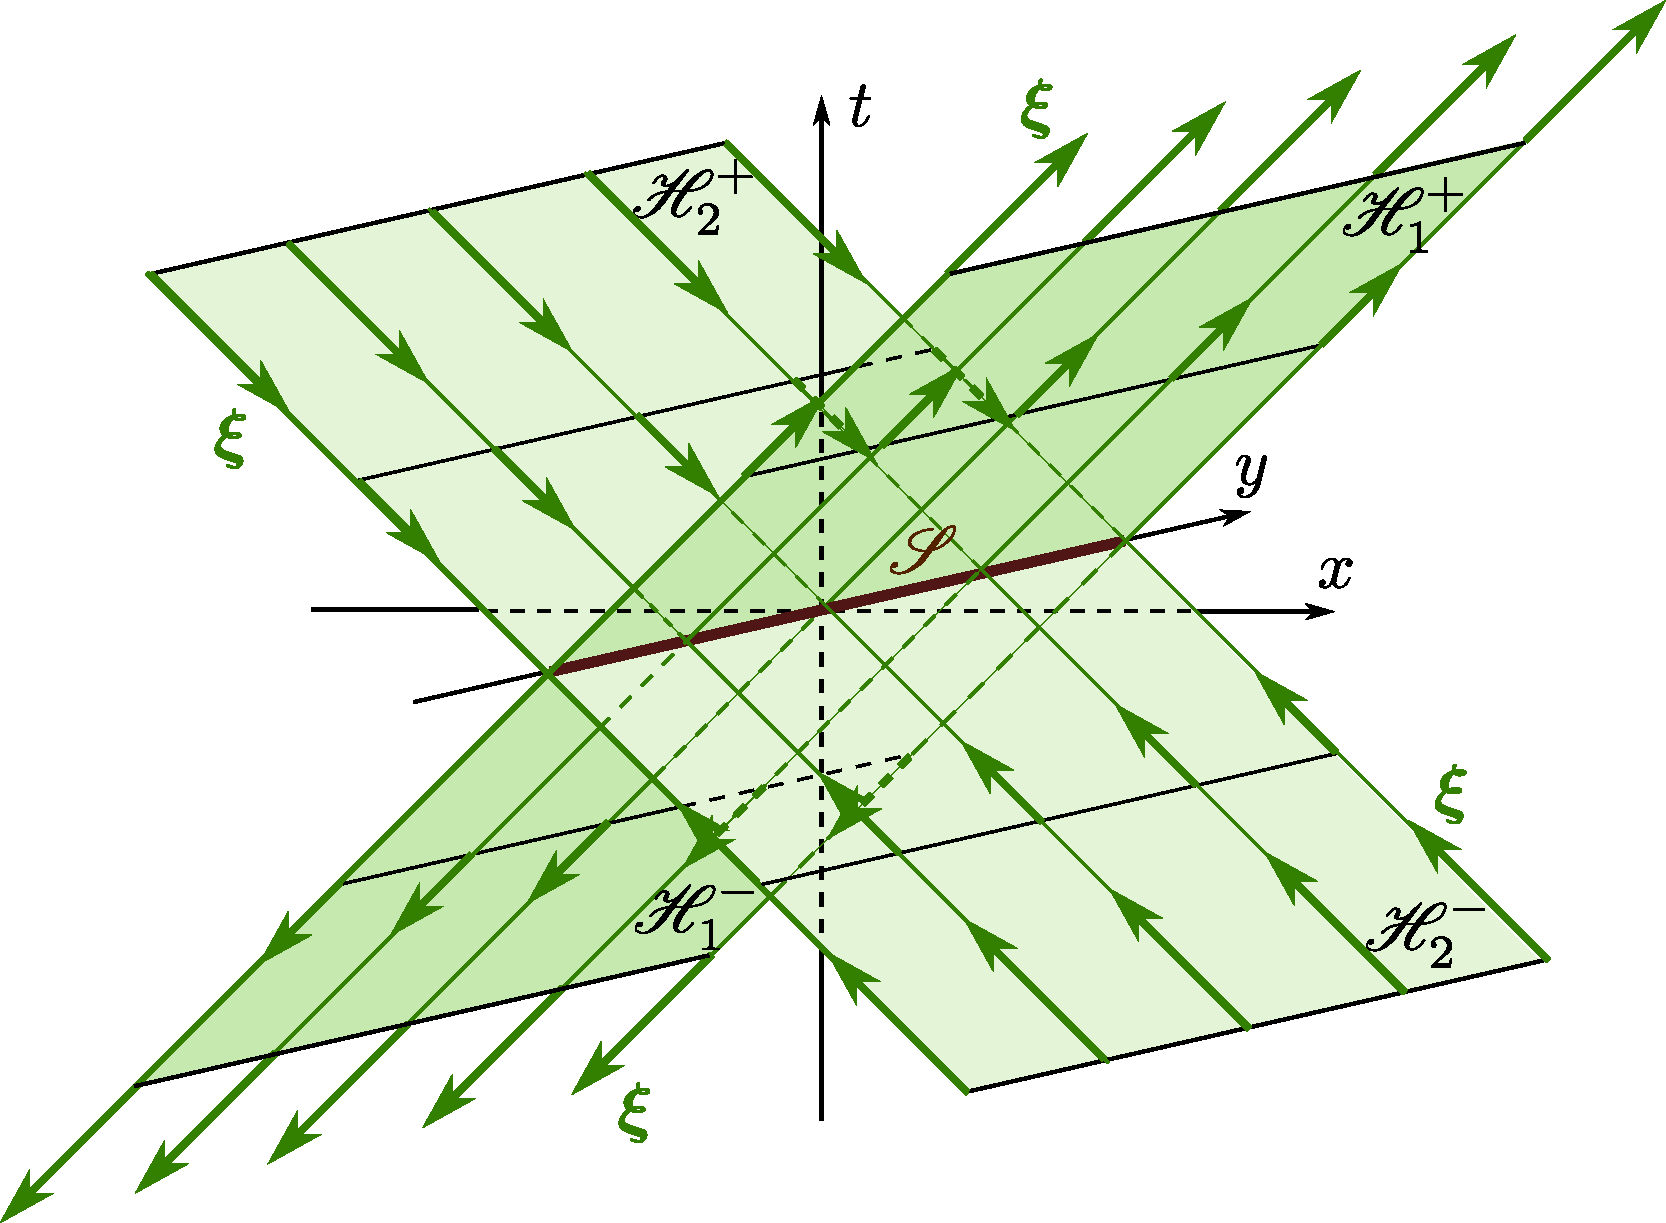
\includegraphics[width=0.6\textwidth]{sta_hplane_bifur.pdf}}
\caption[]{\label{f:sta:hplane_bifur} \footnotesize
Bifurcate Killing horizon $\Hor_1\cup\Hor_2$ with respect to the Killing vector
field $\w{\xi}$ generating Lorentz boosts in the plane $(t,x)$ of Minkowski
spacetime. The dimension along $z$ having been suppressed, the bifurcation
surface $\Sp$ appears as a line, while it is actually a 2-plane.}
\end{figure}

\begin{example}[bifurcate Killing horizon w.r.t. Lorentz boost]
\label{x:sta:bif-KH-boost}
Let us consider the boost Killing vector in Minkowski spacetime as given
by Eq.~(\ref{e:neh:boost-Killing}): $\w{\xi} := x \wpar_t + t \wpar_x$
and let us take for $\Hor_1$ the null hyperplane of equation $t=x$
considered in Example~\ref{x:neh:boostKH} in Chap.~\ref{s:neh} and denoted there
by $\Hor$. The two half-hyperplanes defined by
Eq.~(\ref{e:neh:boost-Killing_hor}) are then the Killing horizons $\Hor_1^+$ and
$\Hor_1^-$. The union $\Hor_1 \cup \Hor_2$, where $\Hor_2$ is the null hyperplane of equation $t=-x$ is a bifurcate Killing horizon with respect to $\w{\xi}$,
with the 2-plane of equation $t=0$ and $x=0$ as the bifurcation surface
(cf. Fig.~\ref{f:sta:hplane_bifur}). Note that on $\Hor_1$, the Killing vector
$\w{\xi}$ points away from $\Sp$, while on $\Hor_2$, it points towards $\Sp$.
\end{example}

\subsection{Non-degenerate Killing horizons and Boyer theorem}

Let us consider a Killing horizon $\Hor$ with respect to some Killing vector
field $\w{\xi}$. As shown in Sec.~\ref{s:neh:zeroth_law},
the surface gravity\index{surface!gravity}  of $\Hor$, i.e.
the non-affinity coefficient $\kappa$ of $\w{\xi}$ on $\Hor$, is constant over
$\Hor$ (the zeroth law of black hole mechanics\index{zeroth law}).
In what follows, we consider the case where $\kappa\not=0$, i.e. $\Hor$
is a non-degenerate Killing horizon (cf. Sec.~\ref{s:neh:classif_KH}).

Let us assume that $\w{\xi}$ is future-oriented on $\Hor$; if not, we can
always consider $\Hor$ as a Killing horizon with respect to $-\w{\xi}$.
Let $t$ be the parameter
associated with $\w{\xi}$ along the null geodesic generators of $\Hor$, i.e.
$\w{\xi} = \D/\D t$ along any null geodesic generator $\Li$.
Since $\kappa\not=0$, $t$ is not an affine parameter of $\Li$.
The null vector field $\wl$ defined on $\Hor$ by
\be \label{e:sta:el_kappa_xi}
    \wl = e^{-\kappa t} \, \w{\xi} \quad \iff\quad
    \w{\xi} = e^{\kappa t} \, \wl
\ee
is a geodesic vector field and the affine parameter associated with it is
\be \label{e:sta:lambda_t}
    \lambda = \frac{e^{\kappa t}}{\kappa} + \lambda_0 ,
\ee
where $\lambda_0$ is a constant.
\begin{proof}
We have
\[
\wnab_{\wl}\, \wl = \wnab_{e^{-\kappa t} \w{\xi}} \left( e^{-\kappa t} \, \w{\xi} \right) = e^{-\kappa t} \wnab_{\w{\xi}} \left( e^{-\kappa t} \, \w{\xi} \right)
= e^{-\kappa t} \big[ \big( \underbrace{\wnab_{\w{\xi}} e^{-\kappa t}}_{\D e^{-\kappa t}/\D t} \big) \w{\xi}
    + e^{-\kappa t} \underbrace{\wnab_{\w{\xi}}\, \w{\xi}}_{\kappa\w{\xi}}
    \big] = 0 .
\]
Hence $\wl$ is a geodesic vector. Besides, along any null generator of $\Hor$,
one has [cf. Eq.~(\ref{e:bas:def_vector})]
\[
    \w{\xi}(\lambda) = \frac{\D\lambda}{\D t} = e^{\kappa t}
    \underbrace{\wl(\lambda)}_{1} = e^{\kappa t} ,
\]
which yields Eq.~(\ref{e:sta:lambda_t}).
\end{proof}
Let us assume $\kappa>0$. Let $\Li$ be a null geodesic generator of the Killing
horizon $\Hor$. $\Li$ can be parametrized by $t$, the corresponding
tangent vector being $\w{\xi}$. When $t$ spans the whole interval $(-\infty,+\infty)$,
Eq.~(\ref{e:sta:lambda_t}) implies that $\lambda$ spans the
interval $(\lambda_0,+\infty)$ only. Since $\lambda$ is an affine parameter of $\Li$,
this means that $\Li$ is an incomplete geodesic.
Moreover, Eq.~(\ref{e:sta:el_kappa_xi}) leads to
\be \label{e:sta:xi_zero_t_inf}
    \w{\xi} \rightarrow 0 \quad\mbox{when}\quad t\rightarrow -\infty \qquad (\kappa>0).
\ee
In other words, the Killing vector field $\w{\xi}$ vanishes and
the null geodesic $\Li$ stops at the ``edge'' of $\Hor$ corresponding to
$t\rightarrow -\infty$. If there is no singularity there, $\Li$ can be
extended to $\lambda\in(-\infty,\lambda_0]$, giving rise to a complete
null geodesic $\tilde L$. This operation can be performed for all the
null geodesic generators of $\Hor$ and we have the freedom to choose the same value
of $\lambda_0$ in Eq.~(\ref{e:sta:lambda_t}) for all of them. In this process,
one gives birth to a null hypersurface, $\tilde\Hor$ say, which contains $\Hor$. Let $\Sp\subset\tilde\Hor$ be the set of points of
affine parameter $\lambda=\lambda_0$ along all the extended null geodesics
$\tilde L$. $\Sp$ is clearly a cross-section of $\tilde\Hor$
(cf. Sec.~\ref{s:def:spacelike_sections}); it is then a
spacelike $(n-2)$-dimensional surface.
$\Sp$ constitutes the past boundary of $\Hor$, i.e. the boundary corresponding to $t\rightarrow -\infty$.
Since $\w{\xi}$ is a smooth vector field on $\M$, Eq.~(\ref{e:sta:xi_zero_t_inf})
implies that $\w{\xi}$ vanishes on $\Sp$.
In other words, $\Sp$ is a set of fixed points for the isometry group generated
by $\w{\xi}$ (cf. Remark~\ref{r:sta:zero_Killing} above).
Let us denote by $\Hor^-$ the subset of $\tilde\Hor$
generated by the segments $\lambda<\lambda_0$ of the null geodesics $\tilde L$:
$\Hor^- = \tilde\Hor\setminus(\Hor\cup\Sp)$.
$\Hor^-$ is clearly a null hypersurface.
Since $\Sp$ is spacelike and $(n-2)$-dimensional, there are, at each point
$p\in\Sp$, only two null directions normal to $\Sp$ (cf. Sec.~\ref{s:def:spacelike_sections}). One of them is along $\wl$. The set of all null geodesics
departing from $\Sp$ along the other null direction forms a null hypersurface,
$\Hor_2^+$ say, in the future of $\Sp$ and another null hypersurface, $\Hor_2^-$
say, in the past of $\Sp$.
By studying the behaviour of a Killing vector field around the set of its
fixed points (here $\Sp$), Boyer \cite{Boyer69} has shown that in
the current setting (i.e. $\Sp$ spacelike), $\w{\xi}$ acts \emph{locally}
as the generator of Lorentz boosts in Minkowski spacetime and $\Sp$ is the bifurcation surface
of a bifurcate Killing horizon similar to that of Example~\ref{x:sta:bif-KH-boost}
(cf. Fig.~\ref{f:sta:hplane_bifur}).
More precisely, Boyer proved the following theorem \cite{Boyer69}:
a Killing horizon $\Hor$ is contained in a bifurcate Killing horizon if and
only if $\Hor$ contains at least one incomplete, extendable, null geodesic
generator. The last property is guaranteed by $\kappa\not=0$, as we have seen.
It follows that $\Hor^-$, $\Hor_2^+$ and $\Hor_2^-$
are three Killing horizons, so that $\Hor\cup\Hor^-\cup\Hor_2^+\cup\Hor_2^-\cup\Sp$
is a bifurcate Killing horizon.

If $\kappa<0$, we see from Eq.~(\ref{e:sta:lambda_t}) that while $t$ spans the
whole interval $(-\infty,+\infty)$, the affine parameter $\lambda$ spans the
interval $(-\infty,\lambda_0)$ only. Moreover Eq.~(\ref{e:sta:el_kappa_xi})
leads to
\be
    \w{\xi} \rightarrow 0 \quad\mbox{when}\quad t\rightarrow +\infty  \qquad (\kappa<0).
\ee
The reasoning developed for $\kappa>0$ can be then applied mutatis mutandis,
leading to a bifurcate Killing horizon with a bifurcation surface $\Sp$ that
is the future boundary of $\Hor$. Hence we conclude
\begin{greybox}
The null geodesic generators of a non-degenerate Killing horizon $\Hor$ are
incomplete; if they can be extended, $\Hor$ is contained in a
bifurcate Killing horizon, the bifurcation surface of which is the past
(resp. future) boundary of $\Hor$ if $\kappa>0$ (resp. $\kappa<0$).
\end{greybox}

\begin{remark}
For a degenerate Killing horizon, the problem of extension disappears, since
$t$ is then an affine parameter of the null generators. Consequently if $t$ spans
the whole interval $(-\infty,\infty)$, the null generators are complete
geodesics. One can still have $\w{\xi}\rightarrow 0$ at some boundary
of $\Hor$, but this is a null boundary, not a spacelike one, and it does not
correspond to a bifurcation surface. An example is the Killing horizon with
respect to a null-rotation Killing vector in Minkowski spacetime, exhibited
as Examples~\ref{x:neh:nullrotKH} and \ref{x:neh:nullrotKH_kappa}
in Chap.~\ref{s:neh}, p.~\pageref{x:neh:nullrotKH} and \pageref{x:neh:nullrotKH_kappa}
respectively (cf. Fig.~\ref{f:neh:hplaneKilling-nullrot}).
\end{remark}

\begin{hist}
The concept of bifurcate Killing horizons has been introduced by Robert H. Boyer\index{Boyer, R.H.}
(1932-1966), a young American mathematical physicist just appointed to the University
of Liverpool and former mathematics instructor at the University of Texas at Austin,
where he died on 1 August 1966, as one of the 14 victims of mass murder.
His last notes, containing the definition of bifurcate Killing horizon
and the proof of the above mentioned theorem, have been transformed to an article
by J. Ehlers and J.L. Stachel and published in 1969 \cite{Boyer69}.
\end{hist}

%%%%%%%%%%%%%%%%%%%%%%%%%%%%%%%%%%%%%%%%%%%%%%%%%%%%%%%%%%%%%%%%%%%%%%%%%%%%%%%

\section{The no-hair theorem}

In dimension $n=4$, one can go much further then just claiming that the
event horizon of a stationary black hole must be a Killing horizon.
One has indeed the \defin{Carter-Robinson theorem}\index{Carter-Robinson theorem}
(Carter 1971 \cite{Carte71}, Robinson 1975 \cite{Robin75}):
any stationary and axisymmetric 4-dimensional asymptotically flat
black hole spacetime $(\M,\w{g})$ that is
solution of the vacuum Einstein equation with a connected regular
event horizon $\Hor$ has a domain of outer communications that is isometric
to the domain of outer communications of the Kerr spacetime.

\begin{remark}
In their original works, Carter and Robinson assumed that $\Hor$ is a
\emph{non-degenerate}
Killing horizon, i.e. that the non-affinity coefficient $\kappa$ associated
with the Killing vector $\w{\chi}$ is non-zero. However this non-degeneracy
hypothesis can be released \cite{ChrusN10} (see \cite{ChrusLH12} for an
extended discussion).
\end{remark}

By combining the staticity, Israel, strong rigidity and Carter-Robinson theorems,
one arrives at the \defin{no-hair theorem}\index{no-hair theorem}:
\begin{greybox}
Any spacetime $(\M,\w{g})$ that
\begin{itemize}
\item is 4-dimensional
\item is asymptotically flat
\item is stationary
\item contains a black hole with a connected regular horizon
\item is analytic
\item is a solution of the vacuum Einstein equation
\end{itemize}
has a domain of outer communications that is isometric
to the domain of outer communications of the Kerr spacetime.
\end{greybox}


